%!TEX root = main.tex

\begin{figure*}[tbp]
	\newcommand\mywidth{0.26}
	\centering
	\subfloat[] {
		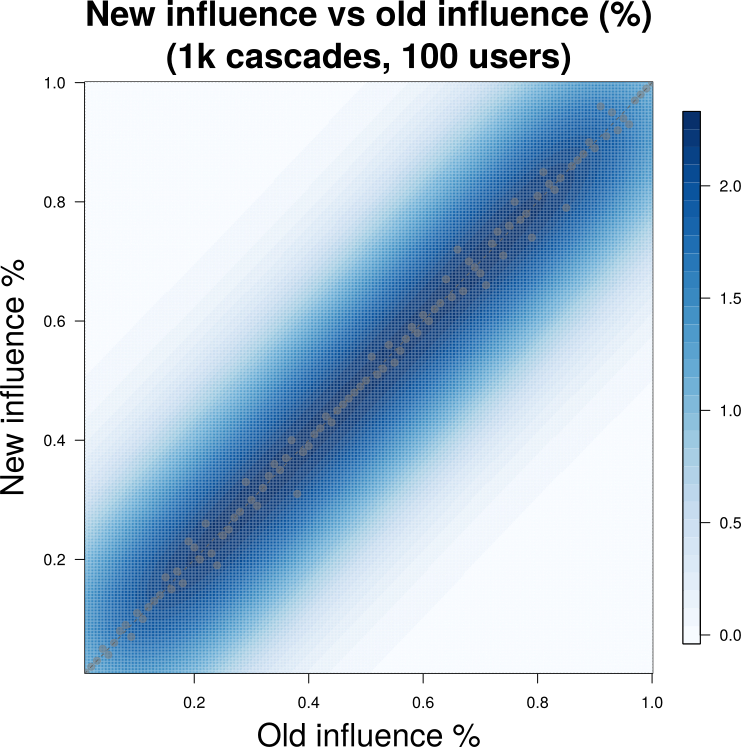
\includegraphics[height=\mywidth\textheight]{1-simulated-data}
		\label{si-fig:new-old-simulated}
	}
%	\hspace{0.15cm}
	\subfloat[] {
		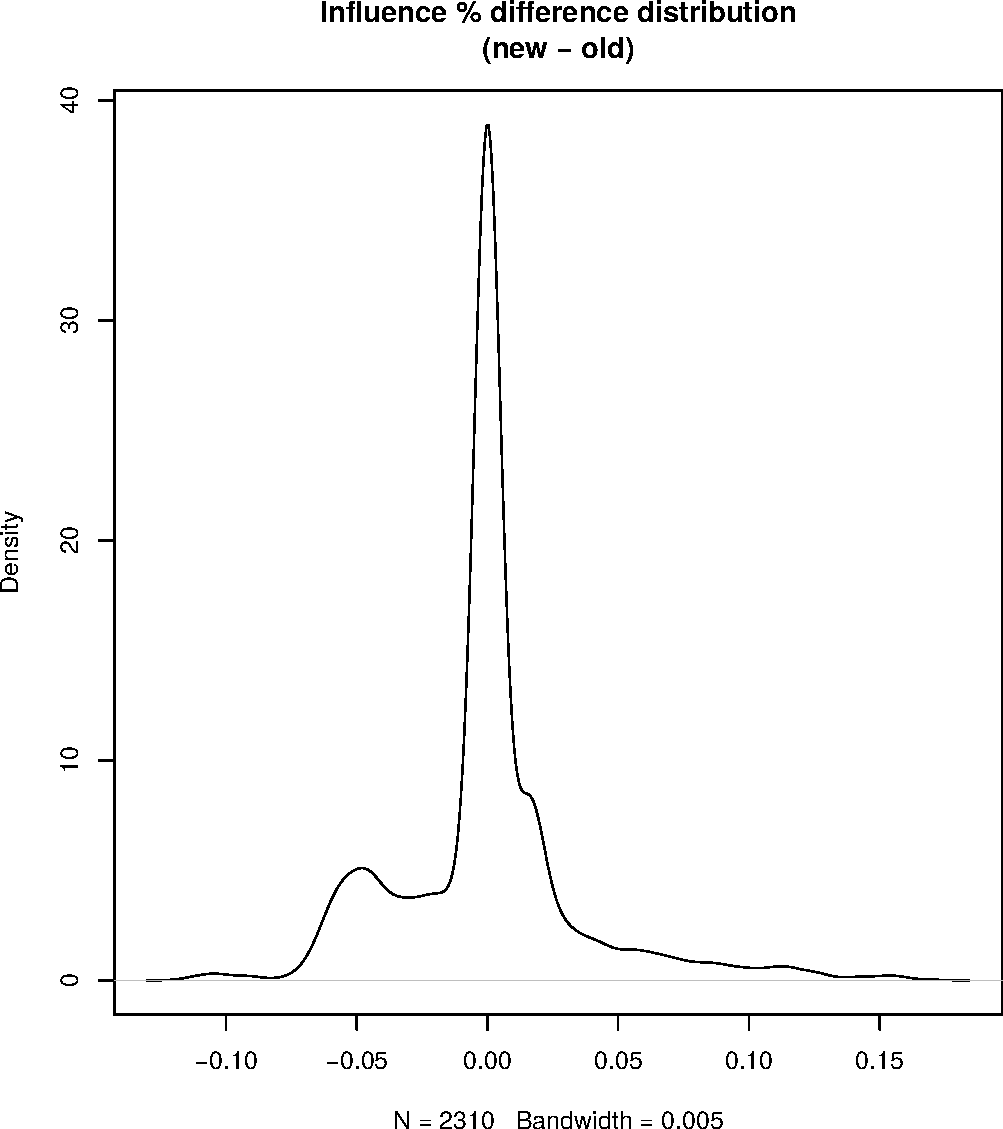
\includegraphics[height=\mywidth\textheight]{2-real-data-diff}
		\label{si-fig:new-old-real-diff}
	}
%	\hspace{0.15cm}
	\subfloat[] {
		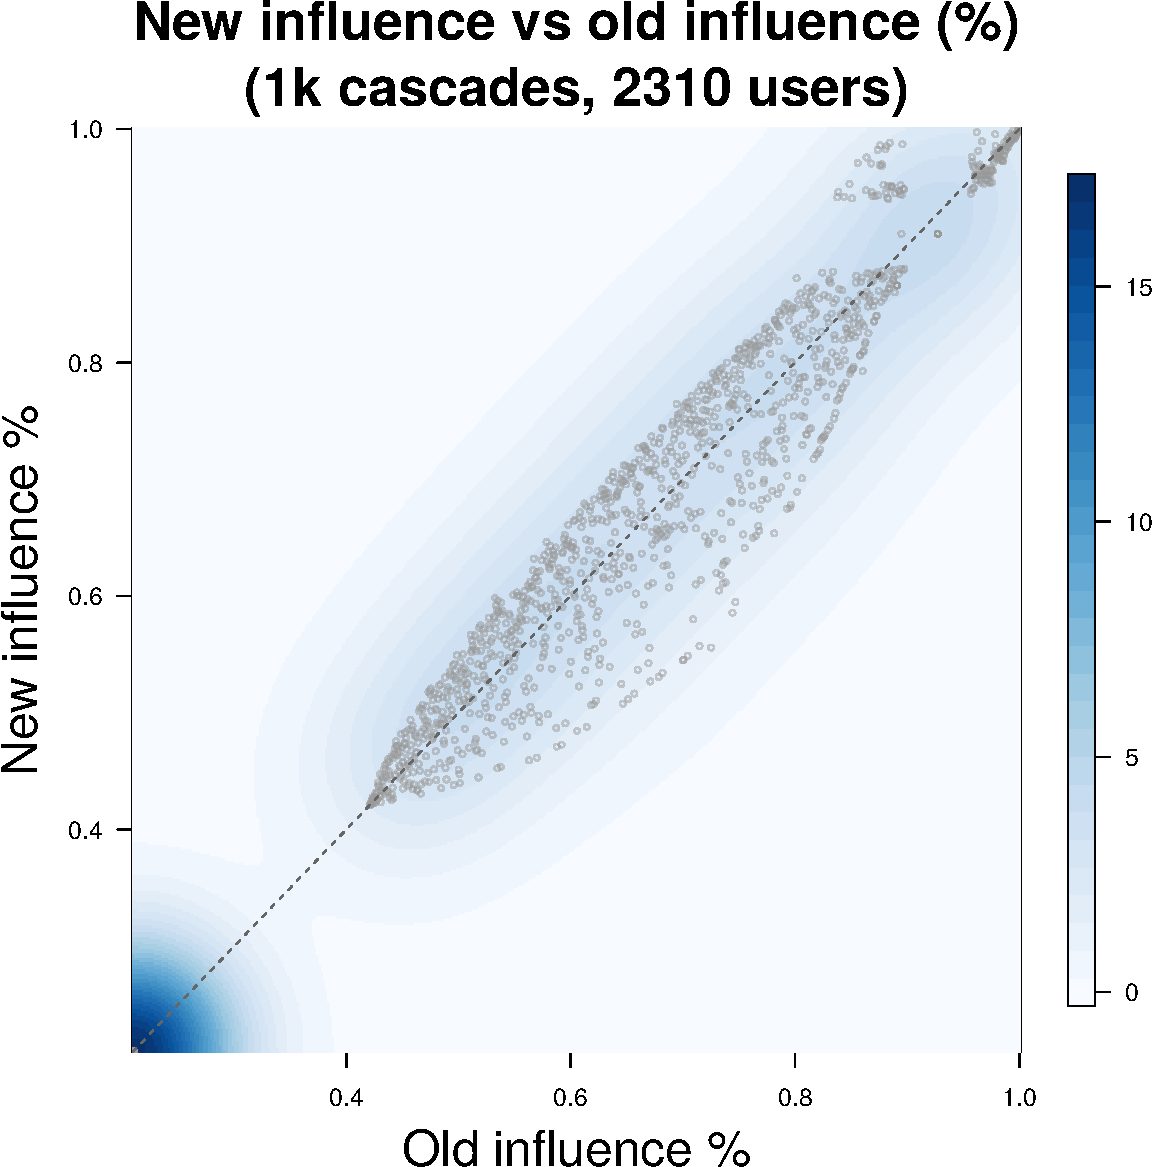
\includegraphics[height=\mywidth\textheight]{3-real-data-2d-plot}
		\label{si-fig:new-old-real}
	}
	\caption{
		Comparison of performances of the algorithm proposed in~\citep{Rizoiu2018a} (i.e. \emph{old}) and our algorithm proposed in Sec.~\ref{si-sec:infl-derivation} and~\ref{si-sec:efficient-algo} (i.e. \emph{new}).
		\textbf{(a)} 2D density plot of the old estimation (on the x-axis) and the new estimation (y-axis).
		100 users participate in 1000 synthetic cascades simulated as described in~\citep{Rizoiu2018a}.
		\textbf{(b)} Distribution of percentile difference and textbf{(c)} 2D density plot between new and old on a sample of 1000 real retweet cascades, containing 2310 users.
	}
	\label{fig:wordclouds}
%	\captionmoveup
\end{figure*}